\subsection{Controller Performance}
The performance of the controller can be tested as in the case of the linear quadratic regulator through simulation, and the result can be seen in \autoref{fig:xbdot_rob} and \ref{fig:yaw_rob}.
%
\begin{figure}[H]
    \captionbox 
    {   
        Step response of the model with the robust controller in $\dot{x}_\mathrm{b}$.
        \label{fig:xbdot_rob}
    }                                                                 
    {                                                                  
        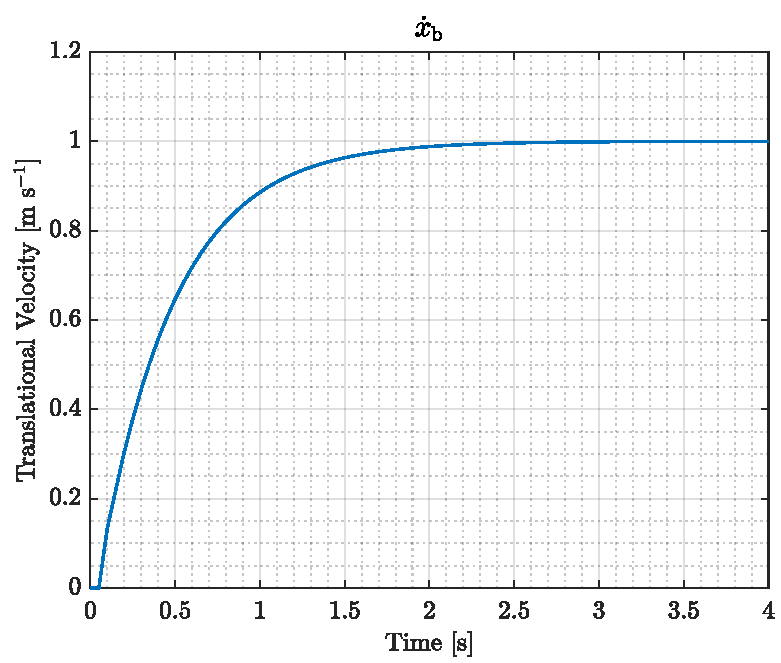
\includegraphics[width=.45\textwidth]{figures/xbdot_rob}         
    }                                                                    
    \hspace{5pt}                                                          
    \captionbox  
    {      
        Step response of the model with the robust controller in $\psi$ at 10 s.
        \label{fig:yaw_rob}
    }                                                                          
    {
        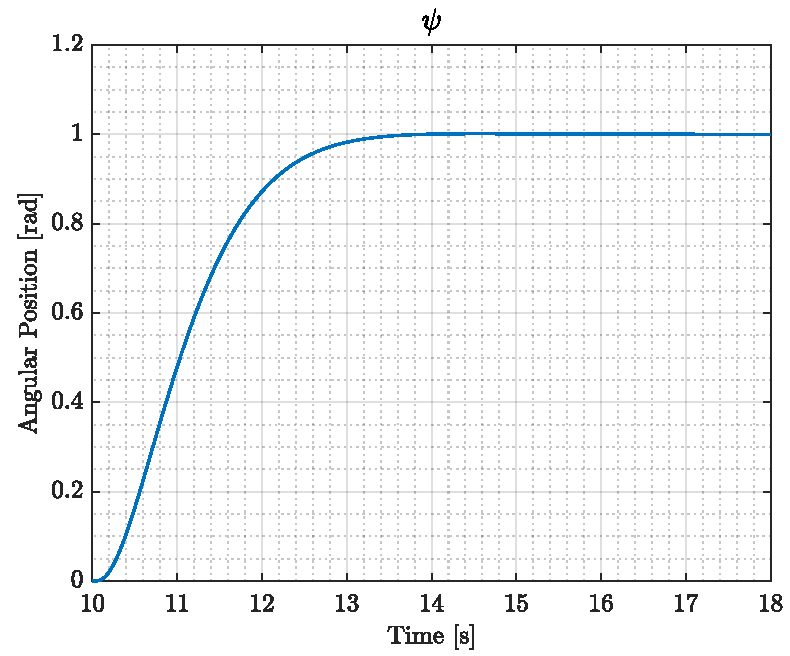
\includegraphics[width=.45\textwidth]{figures/yaw_rob}
    }
\end{figure}
%
\autoref{fig:xbdot_rob} shows the step response of $\dot{x}_\mathrm{b}$, when a reference of 1 m s$^{-1}$ is set. In this case, the settling time is around \num{1.4} s and there is no overshoot.

The response in $\psi$, \autoref{fig:yaw_rob}, shows a settling time of \num{2.6} s and no overshoot.



\fxnote{Check seconds and settling times with final graphs in robust simulations.}